%%%%%%%%%%%%%%%%%%%%%%%%%%%%%%%%%%%%%%%%%%%%%%
% To select a journal, use its code for the 
% journal= option in the \documentclass command.
% The journal codes for this template are:
%
% Antimicrobial Stewardship and Healthcare Epidemiology: ash
% Publications of the Astronomical Society of Australia: pasa
%%%%%%%%%%%%%%%%%%%%%%%%%%%%%%%%%%%%%%%%%%%%%%
\documentclass[
  journal=pasa,
  manuscript=research-paper,
  year=202X,
  volume=YY,
]{cup-journal}

\usepackage{amsmath}
\usepackage{multirow}
\usepackage{amssymb,microtype,siunitx,booktabs}
\sisetup{detect-all,separate-uncertainty=true}
\usepackage{graphicx}
\usepackage{caption}
\usepackage{subcaption}



\title{Synthetic SED Modelling of AGN Contamination in Galaxy Colour-Colour Diagrams}

\author{Mitchell Hooymans}
\affiliation{School of Mathematics and Physics, The University of Queensland, Brisbane, QLD 4072, Australia}
\alsoaffiliation{School of Chemistry and Physics, Queensland University of Technology, Brisbane, QLD 4000, Australia}
\email[Mitchell Hooymans]{m.hooymans@uq.edu.au}

\author{Michael J. Cowley}
\affiliation{School of Chemistry and Physics, Queensland University of Technology, Brisbane, QLD 4000, Australia}
\alsoaffiliation{Centre for Astrophysics, University of Southern Queensland, Toowoomba, QLD 4350, Australia}



\keywords{active galactic nuclei, supermassive black holes, spectral energy distribution, sed modelling, photometry, colour-colour diagrams}

\begin{document}

\begin{abstract}
Active Galactic Nuclei (AGN) emit powerful radiation that can significantly alter the observed light from their host galaxies. This has the potential to bias photometric estimates of galaxy properties and redshift. To investigate this effect, we combine theoretical spectral energy distribution (SED) models with varying AGN contributions and observational data from the FourStar Galaxy Evolution (ZFOURGE) survey. Our analysis reveals that unobscured AGN induce a substantial shift towards bluer colours in both UVJ and ugr colour-colour diagrams. This shift can lead to the misclassification of quiescent galaxies as star-forming and an underestimation of photometric redshifts. Conversely, obscured AGN have minimal impact on these diagnostics. These findings are supported by the analysis of ZFOURGE galaxies, where AGN light is removed via SED fitting and decomposition. Analysis of decomposed ZFOURGE galaxies shows similar behaviour to the theoretical models, with deviations in observational potentially being attributed to intermediate-type AGN, and prompting further research. This study underscores the importance of considering AGN contributions when analysing galaxy properties and evolution, particularly for high-redshift observations from current and future observatories.
\end{abstract}

% ============================================================
\section{INTRODUCTION}
\label{sec:introduction}
% ============================================================

Galaxies exhibit a remarkable diversity in their properties, a key characteristic being star formation activity, broadly distinguishing between actively star-forming galaxies (SFGs) and quiescent galaxies (QGs) \citep{whitaker_newfirm_2011}. This dichotomy is reflected in their colours: SFGs, rich in young, hot stars, typically appear bluer, while QGs, dominated by older stellar populations, are redder \citep{baldry_quantifying_2004}. Galaxy colours provide crucial insights into their underlying physics and evolutionary history, reflecting stellar populations and star formation histories. Young, massive stars emitting predominantly in the UV give SFGs their characteristic blue hue \citep{madau_cosmic_2014}. Declining star formation and stellar evolution/death diminish UV emission, leading to the redder colours of QGs. However, interpreting galaxy colours is complex due to dust obscuration and cosmological redshift.

Further complexity arises from Active Galactic Nuclei (AGN) – compact, luminous galactic cores powered by accreting supermassive black holes (SMBHs). It is thought that these AGN exist at the centre of most massive galaxies and produce intense electromagnetic radiation which can significantly contribute to a galaxy's total light \citep{elvis_atlas_1994}. The contribution of this light to the host's light can affect the observed properties of a galaxy \citep{cowley_decoupled_2018}. In turn this may affect photometric diagnostic diagrams which are vital for galaxy evolution studies. Photometric diagnostic tools offer a rapid, cost-effective alternative to spectroscopy. While less precise, the volume of photometric data allows robust statistical analysis, enabling morphological classification, redshift estimation, and AGN detection. Colour-colour (CC) diagrams are one such photometric diagnostic, which has been used extensively to select AGN \citep{lacy_obscured_2004, messias_dependency_2014, donley_spitzer_2007}, determine redshift \citep{giavalisco_lyman-break_2002}, and to separate star-forming galaxies from quiescent galaxies \citep{whitaker_newfirm_2011}. Therefore AGN light needs to be accounted for when conducting research using photometric techniques. By accounting for AGN light we aim to improve galaxy colour diagnostics for large photometric surveys through quantifying AGN contamination effects on photometric galaxy colours. Through this we aim to enable more accurate analyses of large-scale photometric surveys, ultimately leading to a more complete understanding of galaxy evolution. This research operates within a $\Lambda$CDM cosmological framework, assuming $H_0 = 70$ km s$^{-1}$ Mpc$^{-1}$, $\Omega_M = 0.3$, and $\Omega_{\Lambda} = 0.7$.

% ============================================================
\section{DATA}
\label{sec:data}
% ============================================================

\subsection{Galaxy Templates and AGN Models}
\label{subsec:templates}

To investigate the effect of AGN on their host galaxy, we constructed composite spectral energy distributions (SEDs) by combining galaxy templates with theoretical AGN models. Galaxy templates were drawn from the GALSEDATLAS template library \citep{brown_atlas_2014} due to their extensive wavelength range ($10^2 -$$10^7${\AA}) of 129 nearby galaxies. Rest-frame versions of the galaxy templates were used to eliminate redshift-related effects and ensure consistent comparisons across wavelengths. Theoretical AGN models were selected from the SKIRTOR AGN model set \citep{stalevski_3d_2012, stalevski_dust_2016}, which was chosen for its ability to account for torus orientation and clumpy dust geometry, features that align well with the physical characteristics of AGN emission and have been widely adopted in the literature. The SKIRTOR AGN models simulate AGN emission by utilising the SKIRT code \citep{camps_skirt_2015} to solve the radiative transfer equation and generate an emission spectrum, incorporating a clumpy two-phase dust distribution for the dusty torus. From the SKIRTOR model set (19,200 models), Type 1 and Type 2 AGN models were chosen. To simplify the parameter space, an average AGN model was defined, varying only in inclination to produce Type 1 or Type 2 classifications \citep{ciesla_constraining_2015}. The parameters that were used for the two models are shown in Table \ref{tab:agn_parameters}.

\begin{table}[hbt!]
\begin{threeparttable}
\caption{SKIRTOR AGN Model Parameters}
\label{tab:agn_parameters}
\begin{tabular}{lcc}
\toprule
\headrow Parameter & Type 1 AGN & Type 2 AGN \\
\midrule
Optical Depth & 7 & 7 \\
Radial Gradient & 0.5 & 0.5 \\
Dust Density Gradient & 0 & 0 \\
Opening Angle & 40 degrees & 40 degrees \\
Radius Ratio & 20 & 20 \\
Inclination & 0 degrees & 90 degrees \\
\bottomrule
\end{tabular}
\begin{tablenotes}[hang]
\item[] Parameters used for the Type 1 and Type 2 SKIRTOR AGN models.
\end{tablenotes}
\end{threeparttable}
\end{table}

\subsection{Observational Data}
\label{subsec:obsdata}

This research utilises observational data from the FourStar Galaxy Evolution Survey (ZFOURGE) \citep{straatman_fourstar_2016}. ZFOURGE is a comprehensive photometric imaging survey covering approximately 400 arcmin$^2$ across three \textit{Hubble Space Telescope} (HST) legacy fields: CDFS \citep{giacconi_chandra_2002}, COSMOS \citep{scoville_cosmic_2007}, and UDS \citep{lawrence_ukirt_2007}. Observations were conducted using the FourStar Infrared Camera on the Magellan Baade Telescope at Las Campanas Observatory in Chile \citep{persson_fourstar_2013}. ZFOURGE's strength lies in its deep near-infrared (near-IR) imaging, employing the $J_1$, $J_2$, $J_3$, $H_1$, and $H_2$ medium-band filters, along with the $K_s$ broadband filter. This filter set enables the derivation of highly reliable photometric redshifts, achieving an accuracy of $\Delta z/(1+z) \simeq 1-2\%$ within the redshift range $1 < z < 4$ \citep{straatman_fourstar_2016}. In addition to near-IR coverage, ZFOURGE incorporates multi-wavelength data from several key surveys and observatories. In particular, ZFOURGE utilises data from the Cosmic Assembly Near-infrared Deep Extragalactic Legacy Survey (CANDELS) \citep{koekemoer_candels_2011, grogin_candels_2011, skelton_3d-hst_2014}, providing crucial optical and near-IR information. Data from the \textit{Spitzer Space Telescope} \citep{fazio_infrared_2004, rieke_multiband_2004} further extends the wavelength coverage into the mid-infrared. These data are supplemented by observations from other ground-based telescopes. To facilitate the analysis of active galactic nuclei (AGN), ZFOURGE's multi-wavelength coverage is further enhanced by the inclusion of data from the \textit{Herschel Space Observatory}, the \textit{Chandra X-ray Observatory}, and the \textit{XMM-Newton} space telescope \citep{cowley_zfourge_2016, padovani_active_2017}. This multi-faceted approach allows for the investigation of AGN across a broad range of wavelengths, providing a more complete picture of their properties. Photometric redshifts and rest-frame colours within the ZFOURGE catalogue were calculated using the EAZY code \citep{brammer_eazy_2008}. A comprehensive description of the ZFOURGE data, reduction methods, and photometric bands can be found in \citet{straatman_fourstar_2016}.

% ============================================================
\section{PHOTOMETRIC DIAGNOSTICS}
\label{sec:photometricdiagnostics}
% ============================================================

\subsection{IRAC AGN Selection}
\label{subsec:irac_diagnostic}

A critical prerequisite for advancing our understanding of AGN feedback mechanisms is the accurate differentiation between active and inactive galaxies. Many detection and selection methodologies exist, ranging from X-ray emission analysis \citep{szokoly_chandra_2004}, emission-line diagnostics utilising Baldwin-Phillips-Terlevich diagrams (BPT) \citep{baldwin_classification_1981}, and radio activity assessment \citep{rees_radio_2016}. However, these techniques exhibit inherent limitations, often involving substantial observational resources, intricate data reduction procedures, and potential biases. The approach for selecting AGN that is focused on in this paper utilises the mid- to near-infrared photometry selection technique first used by \cite{lacy_obscured_2004} which leverages the characteristic thermal emission from hot dust surrounding the AGN. The Lacy wedge implemented in this study uses the following criteria:
\begin{align*}
    \log_{10}\left(f_{5.8}/f_{3.6}\right) &> -0.1\\
    \log_{10}\left(f_{8.0}/f_{4.5}\right) &> -0.2\\
    \log_{10}\left(f_{8.0}/f_{4.5}\right) &< 0.8 \times \log_{10}\left(f_{5.8}/f_{3.6}\right) + 0.5
\end{align*}

\subsection{UVJ Star-formation Classification}
\label{subsec:uvj_diagnostic}

To investigate how AGN affect galaxy populations we use the UVJ diagram which categorises galaxies by their star formation and infer their morphology can be done using the UVJ colour-colour diagram. This diagnostic tool relies on using the rest-frame U-V and V-J colours which reflect a galaxy's ultraviolet, optical and near-infrared photometry. The UVJ diagram can be used to identify dust-obscured galaxies, and the use of rest-frame colours ensures a selection where redshifting effects have been minimised. The UVJ diagram works by exploiting the colour bimodality between star-forming and quiescent galaxies, where star-forming galaxies appear bluer, while quiescent galaxies appear redder. In general, this colour bimodality can also be used as a proxy for a galaxy's morphological structure, as star-forming galaxies in general have longer periods of sustained star formation, and appear bluer, while elliptical galaxies generally exhaust their fuel for star formation and more quickly appear red. This UVJ selection works by dividing the UVJ diagram into regions of star formation, quiescence and dust. The UVJ diagram is split into three distinct regions.

The quiescent region is defined by:
\begin{align*}
    (V - J, U - V) \geq (-\infty, 1.3), (0.85, 1.3), (1.6, 1.95), (1.6, +\infty)\\
\end{align*}
The remaining regions were defined by being located outside the quiescent selection region. The star-forming region is defined by:
\begin{align*}
    (V - J, U - V) &\leq (-\infty, 1.3), (0.85, 1.3), (1.6, 1.95), (1.6, +\infty)\\
    (V - J) &\leq 1.2
\end{align*}
The dusty region is given by:
\begin{align*}
 (V - J, U - V) &\leq (-\infty, 1.3), (0.85, 1.3), (1.6, 1.95), (1.6, +\infty)\\
    (V - J) &\geq 1.2
\end{align*}

% ============================================================
\section{METHODOLOGY}
\label{sec:methodology}
% ============================================================

\subsection{Constructing Composite SEDs}
\label{subsec:compositeseds}

To investigate the effect of AGN on photometric diagnostics, a simplified composite model was used, where the energetic output is a linear combination of its AGN and galaxy components. The composite SED is described by:
\begin{align*}
f_{\lambda, total}(\lambda) = f_{\lambda, Galaxy}(\lambda) + \alpha \cdot f_{\lambda, AGN}(\lambda)
\end{align*}
Here, $f_{\lambda}(\lambda)$ represents the SED of a source, and $\alpha$ denotes the fraction of the AGN SED present in the total galaxy SED. To create composite SEDs, galaxy and AGN models were aligned and scaled. SED alignment involved matching wavelength ranges and using linear interpolation to estimate missing flux values, ensuring consistent wavelength coverage. Integral normalisation was applied to scale the chosen AGN model to the desired galaxy template using the integrated flux:
\begin{align*}
F_{\lambda} = \int_{\lambda_{min}}^{\lambda_{max}} f_\lambda(\lambda) d\lambda
\end{align*}
The integrated flux, $F_{\lambda}$, was calculated for both galaxy and AGN and was used to choose the scaling factor, $SF$:
\begin{align*}
SF = \frac{F_{\lambda, \text{Galaxy}}}{F_{\lambda, \text{AGN}}}
\end{align*}
This scaling was applied to the AGN SED which gives the final composite SED equation as:
\begin{align*}
f_{\lambda, \text{total}}(\lambda) = f_{\lambda, \text{Galaxy}}(\lambda) + \alpha \cdot (f_{\lambda, \text{AGN}}(\lambda) \cdot SF)
\end{align*}
In creating SED composites, $\alpha$ varied from 0 to 1 in steps of 0.1, resulting in 10 composite SEDs for each galaxy-AGN combination. This range was chosen to explore a variety of AGN contributions, including those of low-luminosity AGNs in host galaxies.

\subsection{Synthetic Photometry and Colour-Space Construction}
\label{subsec:syntheticphot}

A comprehensive set of composite SEDs was constructed, encompassing all galaxy templates combined with both Type 1 and Type 2 AGN models. Synthetic photometry was then derived from these composite SEDs, allowing for the creation of colour-colour diagrams. To quantify the impact of AGN contamination, we apply two commonly used photometric diagnostics to our synthetic photometry: the UVJ diagram for star formation classification and the IRAC colour space for AGN selection. Each diagnostic uses rest-frame colours derived from our composite SEDs.

\subsection{Quantifying Contamination via Mean Vector Offset}
\label{subsec:vectoroffset}

To quantify the change in position for each composite type, the average position for all sources within the colour-colour diagram was calculated at each $\alpha$ value. A vector offset was used to measure the movement from the initial position with increasing AGN contribution.

% ============================================================
\section{RESULTS}
\label{sec:results}
% ============================================================

\subsection{Model Validation via IRAC Colour Space}
\label{subsec:irac_results}

Mid-infrared colours have long been used to select AGN in large photometric surveys. To that end, the IRAC colour-colour diagram was used to identify if the AGN models were effectively behaving as they did in observation. In Figure~\ref{fig:Brown-IRAC-combined}(a), the effect of Type 1 AGN composites on the IR colour space is explored. By increasing AGN contribution, galaxies systematically move outside of the selection region. This is reflected in the completeness value, which is reduced from 0.26 to 0.06 as the AGN contribution increases from 0\% to 100\%.

While the IRAC diagram shows a clear removal of sources from the selection region for Type 1 AGN composites, Type 2 composites show the opposite effect (see Figure~\ref{fig:Brown-IRAC-combined}(b)). Increasing the AGN contribution in these composites leads to a dramatic rise in the completeness of the selection wedge, bringing a substantial number of sources into the selection region. With an AGN contribution of 70\%, over 98\% of sources fall within this region. The models replicate the expected behaviour of a Type 2 AGN, which is consistent with the design of the Lacy selection region, which was designed to select obscured AGN due to their thermally produced IR emissions from the dusty torus \citep{lacy_obscured_2004, lacy_optical_2007}. The Type 1 AGN composites exhibited a contrasting behaviour, clustering outside the selection region and demonstrating a significant decrease in completeness. This clustering and reduced completeness is likely attributed to the higher emissions in the shorter end of the MIR range, characteristic of Type 1 AGN \citep{thorne_deep_2022}, resulting in `bluer' IRAC colours than those produced by a Type 2 AGN.

\begin{figure*}[t!]
    \centering
    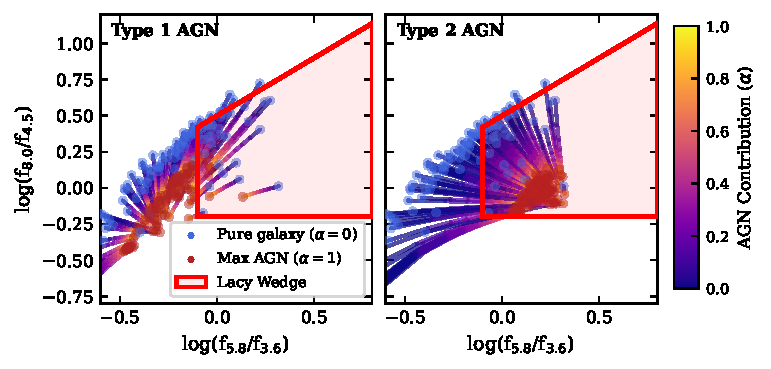
\includegraphics[width=\linewidth]{Images/TheoreticalModelPlots/Paper_IRAC_Evolution_Combined.pdf}
    \caption{Colour evolution tracks in the IRAC diagram for Type 1 (a) and Type 2 (b) AGN composite SEDs constructed using the GALSEDATLAS templates. Track colour encodes AGN contribution from $\alpha=0$ (dark purple) to $\alpha=1$ (yellow). Blue circles mark the pure galaxy starting position; red circles mark the maximum AGN contribution. The red shaded region is the Lacy AGN selection wedge.}
    \label{fig:Brown-IRAC-combined}
\end{figure*}

Table \ref{tab:irac_vectoroffset} shows the mean displacement for each composite set. Unlike the UVJ colour space, there is an apparent increase in displacement for both Type 1 and Type 2 AGN composites across all AGN contributions. Notably, this increase is more pronounced in Type 2 composites compared to Type 1. At 100\% AGN contribution, the displacement reaches 0.36 dex for Type 1 and 0.61 dex for Type 2 composites.

\begin{table}[h!]
\begin{threeparttable}
\caption{Mean Vector Offsets from the initial position for both AGN Composite Model Types and AGN Contribution amounts for IRAC composites.}
\label{tab:irac_vectoroffset}
\begin{tabular}{lcc}
\toprule
\headrow AGN Contribution (\%) & Type 1 Composite & Type 2 Composite \\
\midrule
10  & 0.09 & 0.23 \\
20  & 0.15 & 0.34 \\
30  & 0.19 & 0.41 \\
40  & 0.23 & 0.46 \\
50  & 0.26 & 0.50 \\
60  & 0.29 & 0.53 \\
70  & 0.31 & 0.56 \\
80  & 0.33 & 0.57 \\
90  & 0.34 & 0.59 \\
100 & 0.36 & 0.61 \\
\bottomrule
\end{tabular}
\end{threeparttable}
\end{table}

\subsection{UVJ Colour Evolution}
\label{subsec:uvj_results}

\subsubsection{Type 1 AGN}
\label{subsubsec:type1uvj}

\begin{figure*}[t!]
    \centering
    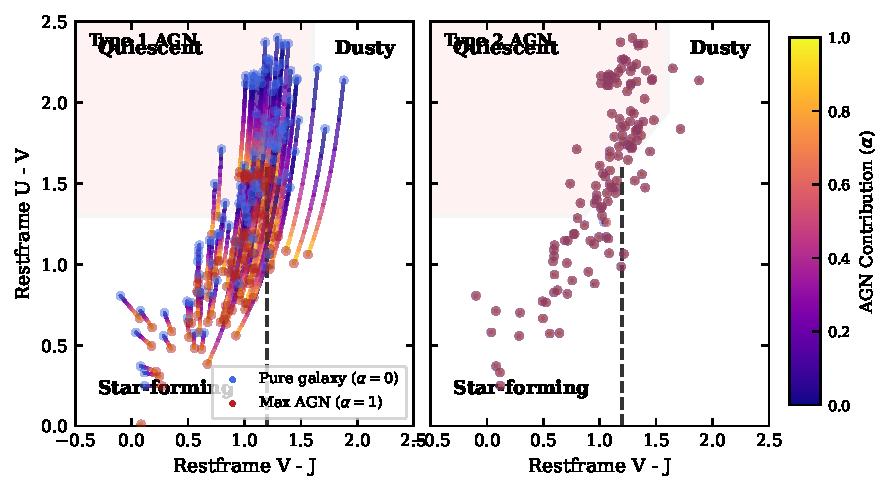
\includegraphics[width=\linewidth]{Images/TheoreticalModelPlots/Paper_UVJ_Evolution_Combined.pdf}
    \caption{UVJ colour-colour evolution tracks for Type 1 (a) and Type 2 (b) AGN composite SEDs constructed from the GALSEDATLAS templates. Track colour encodes AGN contribution from $\alpha=0$ (dark purple, blue circles) to $\alpha=1$ (yellow, red circles). Type 1 composites show a clear systematic shift towards the star-forming region; Type 2 composites exhibit minimal colour evolution.}
    \label{fig:Brown-UVJ-combined}
\end{figure*}

Figure~\ref{fig:Brown-UVJ-combined}(a) illustrates the UVJ colour evolution of a Type 1 AGN composite as the AGN contribution increases. We observe a clear trend of sources moving toward the star-forming region of the UVJ diagram. The galaxy population fraction is located in each region of the UVJ diagram and corresponds to the fraction of galaxies from all sources within a particular region. We see in the theoretical model that there is a higher fraction of quiescent galaxies within the UVJ diagram at low alpha values. However, as the AGN contribution increases, the quiescent fraction drops. In contrast, the dusty fraction slightly increases, and the star-forming fraction drastically increases. The inclusion of a Type 1 AGN component caused a drastic drop in the quiescent fraction of galaxies, whereby quiescent selected sources moved into the star-forming region of the UVJ diagram. The cause of this is due to the increased UV radiation that is being picked up by the U band in the SED (See Figure \ref{fig:composite_uvj}). This increase in ultraviolet radiation is characteristic of Type 1 AGN in which the central accretion disc produces short wavelength emissions in the UV and X-ray bands \citep{nour_association_2023}. As quiescent composites contain higher AGN components, they will eventually be misidentified by the UVJ diagram as star-forming sources, drastically affecting the identification of quiescent type galaxies within the colourspace due to their extremely blue colours \citep{florez_exploring_2020}.

The population fraction evolution with increasing AGN contribution is illustrated in Figure~\ref{fig:uvj-fractions-combined} for both Type 1 and Type 2 composites. A 10\% Type 1 AGN contribution shifts the average UVJ position by 0.09 dex, with the average displacement reaching 0.52 dex at 100\% AGN contribution.

\begin{figure}[h!]
    \centering
    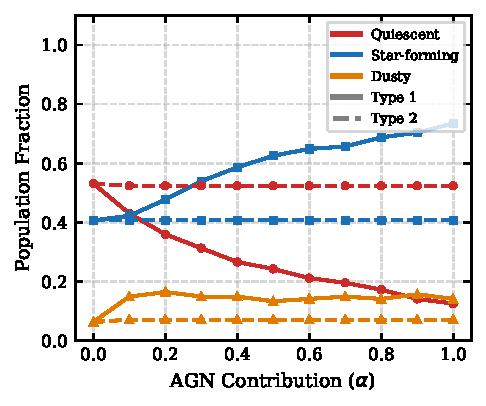
\includegraphics[width=\linewidth]{Images/TheoreticalModelPlots/Paper_UVJ_Fractions_Combined.pdf}
    \caption{UVJ population fractions as a function of AGN contribution ($\alpha$) for Type 1 (solid lines) and Type 2 (dashed lines) composites. For Type 1, the quiescent fraction (red) declines sharply with increasing AGN contribution while the star-forming fraction (blue) rises correspondingly; the dusty fraction (amber) shows only a modest increase. Type 2 composites show no significant change across all fractions, consistent with the minimal colour evolution expected from an obscured AGN.}
    \label{fig:uvj-fractions-combined}
\end{figure}

\subsubsection{Type 2 AGN}
\label{subsubsec:type2uvj}

Incorporating a Type 2 AGN contribution yields no substantial change in the overall galaxy fractions of the composites, except for a minor reduction in the quiescent fraction accompanied by a corresponding 1\% increase in the dusty fraction. Unlike the Type 1 composite, the Type 2 composite did not significantly impact the colours of the sources in the UVJ diagram. In Figure~\ref{fig:Brown-UVJ-combined}(b), there is almost no movement in the UVJ diagram, nor is there any significant change to the galaxy fractions. This is because Type 2 AGN are obscured sources that thermally reprocess much of their UV-Optical emissions into the MIR \citep{padovani_active_2017}. The UVJ filter system, encompassing ultraviolet, optical, and near-infrared wavelengths, lacks the sensitivity to detect changes induced explicitly by obscured AGN activity.

In contrast, Type 2 composites exhibited no discernible change in their average UVJ position, as seen in Figure~\ref{fig:uvj-fractions-combined}. Ultimately, Type 1 AGN composites exhibit a characteristic shift towards the star-forming region with increasing AGN contribution, while Type 2 AGN composites remain largely stationary in the UVJ diagram at all AGN contributions.

\begin{figure*}[t!]
    \centering
    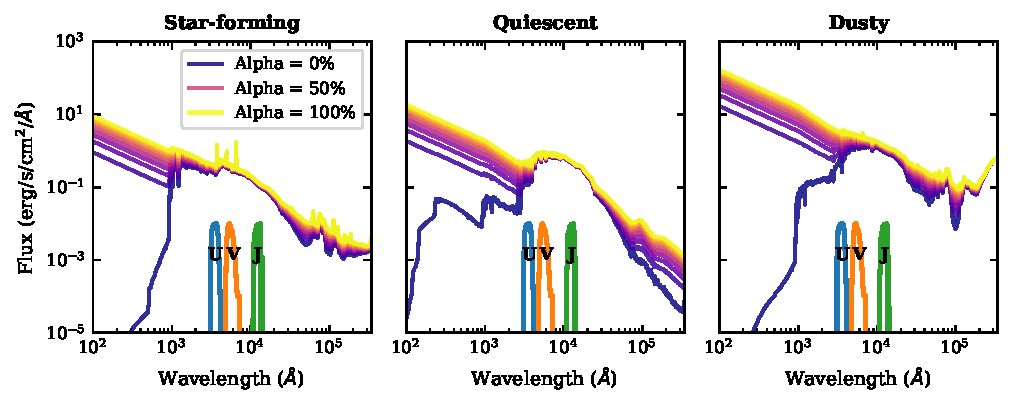
\includegraphics[width=\linewidth]{Images/TheoreticalModelPlots/CompositeSEDs_UVJ.pdf}
    \caption{Rest-frame Type 1 AGN composite SEDs for representative galaxies from the Star-forming (NGC 0337), Quiescent (NGC 4552), and Dusty (IC 4553) regions of the UVJ diagram. Each panel shows the progression from the pure host galaxy SED (purple) to the AGN-dominated composite (yellow), with the plasma colourmap gradient indicating increasing AGN contribution from 0\% to 100\%.}
    \label{fig:composite_uvj}
\end{figure*}

\subsection{Observational Validation with ZFOURGE}
\label{subsec:zfourge_validation}

These theoretical trends are confirmed by the observational ZFOURGE data. Figure \ref{fig:ZFOURGE-EAZY-UVJ} shows four snapshots of the UVJ density distribution for the ZFOURGE sample at AGN contributions of 0\%, 30\%, 70\%, and 100\%. The initial density distribution reveals a substantial concentration of points within the star-forming region. As AGN contribution increases, sources on the outer edge of this density plot, especially those in the quiescent region, gradually move towards the region of highest density. This migration leads to a decrease in quiescent and dusty fractions, accompanied by a corresponding increase in the star-forming fraction, mirroring the observations made using the GALSEDATLAS templates.

\begin{figure*}[t!]
    \centering
    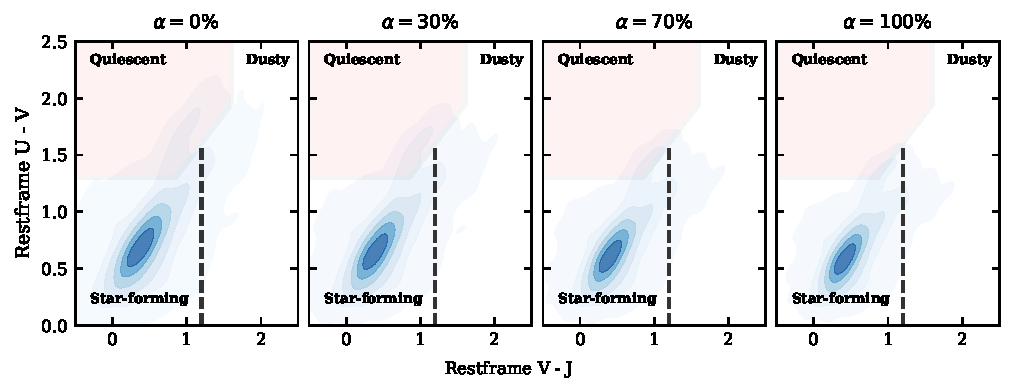
\includegraphics[width=\linewidth]{Images/TheoreticalModelPlots/UVJ_Type1_Density_Evolution.pdf}
    \caption{UVJ density evolution for Type 1 AGN composites applied to the ZFOURGE observational sample ($\sim$11,000 galaxies), showing snapshots at AGN contributions of 0\%, 30\%, 70\%, and 100\%. Each panel shows the density of galaxy positions in UVJ colour space. The progressive shift away from the quiescent region and towards the star-forming region is evident as AGN contribution increases.}
    \label{fig:ZFOURGE-EAZY-UVJ}
\end{figure*}

The observed over-density within the star-forming region of Figure \ref{fig:ZFOURGE-EAZY-UVJ} necessitates considering region-specific colour evolution paths. Figure \ref{fig:ZFOURGE-EAZY-UVJSingleGalaxy_Comparison} illustrates this, showcasing the colour evolution of composite sources at the average position of each population of sources. Star-forming galaxies exhibit minimal colour shifts, while quiescent and dusty galaxies undergo substantial changes. While each population shifts positions, an average galaxy stays within the respective selection regions, even at high AGN contribution amounts.

\begin{figure*}[t!]
    \centering
    \begin{subfigure}[b]{0.48\linewidth}
        \centering
        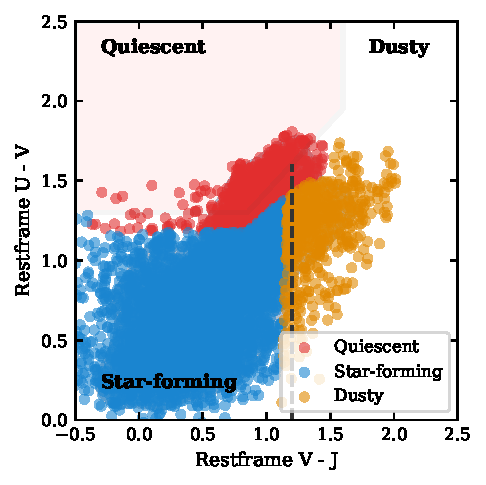
\includegraphics[width=\textwidth]{Images/TheoreticalModelPlots/ZFOURGE_UVJ_Density_alpha50.pdf}
    \end{subfigure}
    \hfill
    \begin{subfigure}[b]{0.48\linewidth}
        \centering
        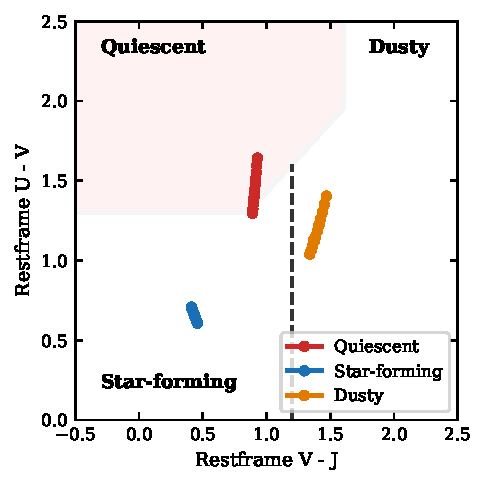
\includegraphics[width=\textwidth]{Images/TheoreticalModelPlots/ZFOURGE_UVJ_RegionTracks.pdf}
    \end{subfigure}
    \caption{Left: UVJ scatter of ZFOURGE galaxies at 50\% AGN contribution, colour-coded by initial UVJ classification (Quiescent: red, Star-forming: blue, Dusty: amber) with KDE density overlay. Right: mean colour evolution tracks for each population as AGN contribution increases from 0\% to 100\%, with arrows indicating the direction of motion.}
    \label{fig:ZFOURGE-EAZY-UVJSingleGalaxy_Comparison}
\end{figure*}

The vector offsets are region-dependent. The star-forming region demonstrates a maximum shift of 0.1 dex at 100\% AGN contribution. In contrast, both the quiescent and dusty populations exhibit a more pronounced positional change, shifting by approximately 0.04 dex for every 10\% increase in AGN contribution within the composite spectra, with maximum offsets of 0.32 and 0.36 dex, respectively. An increase in AGN contribution significantly alters the UVJ colours of galaxies, particularly those near the star-forming/quiescent boundary, as the GALSEDATLAS templates were constructed from real galaxy spectra which inherently include contributions from intrinsic AGN activity \citep{brown_atlas_2014}.

SED decomposition via CIGALE provides observational support for these theoretical predictions. In Figure \ref{fig:uvj-cigale-comparison}, removing the AGN component causes a noticeable increase in the quiescent fraction and a proportionate decrease in the star-forming fraction, a behaviour observed in the previous two sections. This reddening effect aligns with composite models where adding an AGN leads to a bluer galaxy characterised by a reduced quiescent fraction and an increased star-forming fraction. Removing the AGN component revealed a noticeable shift in the colours of the sources.

\begin{figure}[h!]
    \centering
    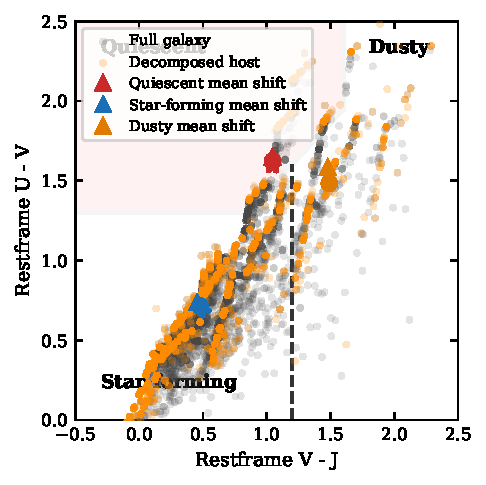
\includegraphics[width=\columnwidth]{Images/TheoreticalModelPlots/UVJ_CIGALE_FullDecomp_Vectors.pdf}
    \caption{UVJ diagram showing the shift between full galaxy colours (dark circles, including AGN light) and CIGALE-decomposed host colours (orange triangles, AGN removed). Bold coloured arrows show the mean displacement per UVJ population — red (Quiescent), blue (Star-forming), amber (Dusty) — computed separately to account for the overdensity in the star-forming region. Removing the AGN component causes a systematic shift towards redder, quiescent colours across all populations.}
    \label{fig:uvj-cigale-comparison}
\end{figure}

Figure \ref{fig:redshift-comparison} shows the average UVJ point throughout different redshift bins, both with and without an AGN component. Both the complete UVJ colours and the decomposed UVJ colours share similar positions at low redshifts but begin to diverge at a redshift bin of 1.4 to $\sim$2, with the effect becoming more prominent at redshifts greater than 2.

\begin{figure}[h!]
    \centering
    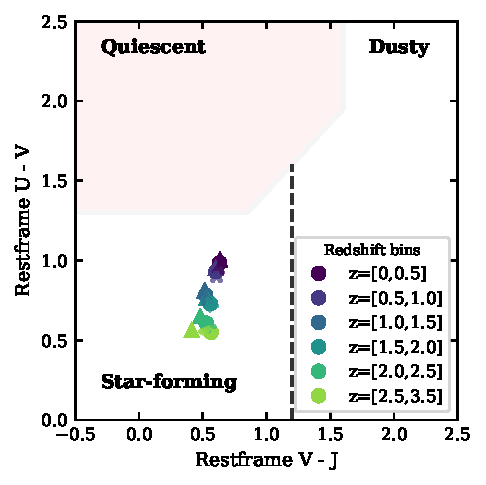
\includegraphics[width=\columnwidth]{Images/TheoreticalModelPlots/UVJ_agn_evolution_CIGALE_ZFOURGE_comparison_redshift.pdf}
    \caption{The UVJ Diagram shows a scatter plot of all sources. In this plot, the average location for each redshift bin is plotted. The full galaxies that include their AGN component are plotted as circles, while the decomposed galaxies that have their AGN removed have been plotted as triangles. Errors have been averaged for each redshift from all sources and propagated from the error in ZFOURGE.}
    \label{fig:redshift-comparison}
\end{figure}

% ============================================================
\section{DISCUSSION}
\label{sec:discussion}
% ============================================================

\subsection{AGN Contamination in the UVJ Diagram}
\label{subsec:disc_contamination}

The most significant difference in the SED lies in the flux observed around the U filter at around 3500\,\AA\ for quiescent and dusty galaxies compared to star-forming galaxies (See Figure \ref{fig:composite_uvj}). Incorporating an AGN component increases the flux in this wavelength range for dusty and quiescent galaxies, which is then picked up by the UVJ filters. The inclusion of a Type 1 AGN component caused a drastic drop in the quiescent fraction of galaxies, whereby quiescent selected sources moved into the star-forming region of the UVJ diagram. As quiescent composites contain higher AGN components, they will eventually be misidentified by the UVJ diagram as star-forming sources, drastically affecting the identification of quiescent type galaxies within the colourspace due to their extremely blue colours \citep{florez_exploring_2020}.

\subsection{Comparison of Theoretical and Observational Results}
\label{subsec:disc_comparison}

While the UV shift aligns with theoretical predictions, the VJ shift shows a significant deviation. As depicted in Figure \ref{fig:uvj-cigale-comparison}, this pronounced VJ shift could be attributed to the absence of intermediate-type AGN in the models. These AGN, with their line-of-sight aligned with the dusty torus opening angle, are expected to exhibit substantial mid-infrared (MIR) emission \citep{ciesla_constraining_2015}, potentially leading to a VJ shift and subsequent misclassification as a dusty source.

Decomposed galaxy colours tend to shift towards the dusty region of the UVJ colourspace, particularly at high redshifts where the offset significantly exceeds the uncertainty for each bin. Despite these potential issues, the full and decomposed galaxy samples follow the expected evolutionary trend. Galaxies appear more star-forming at higher redshifts and become increasingly quiescent towards the present day, consistent with our current understanding of cosmic star-formation history \citep{madau_cosmic_2014, kim_cosmic_2024}.

\subsection{Limitations and Future Work}
\label{subsec:disc_limitations}

While this technique was useful for AGN selection, requiring only three photometric bands, there are certain downsides. The Lacy wedge was designed to identify AGN through their distinctive IR colours and is susceptible to contamination from star-forming galaxies exhibiting strong mid-infrared emission due to Polycyclic Aromatic Hydrocarbons (PAH; \citealt{sajina_simulating_2005}). It is worth noting that while the Lacy Wedge was used to validate AGN candidates, it is prone to high contamination and does not effectively select Type 1 AGN \citep{donley_identifying_2012}. Future work may benefit from the use of a different IR colour space to probe both Type 1 and Type 2 AGN effects; this could be done with either the KI and KIM methods \citep{messias_new_2012, messias_dependency_2014} or by using WISE colours \citep{caccianiga_wise_2015}.

The ugr and UVJ diagrams generated from the ZFOURGE data using CIGALE exhibit a prominent pattern of striations, particularly noticeable when the AGN component is removed. As the striations became more noticeable once the AGN component was removed, the most likely explanation is due to degeneracies in the SED parameters during the CIGALE fitting procedure \citep{yang_x-cigale_2020}.

% ============================================================
\section{CONCLUSIONS}
\label{sec:conclusions}
% ============================================================

\newpage
\paragraph{Acknowledgments}
We are grateful for the technical assistance of A. Author.

\paragraph{Funding Statement}
This research was supported by grants from the <funder-name><doi>(<award ID>); <funder-name><doi>(<award ID>).

\paragraph{Competing Interests}
A statement about any financial, professional, contractual or personal relationships or situations that could be perceived to impact the presentation of the work --- or `None' if none exist

\paragraph{Data Availability Statement}
A statement about how to access data, code and other materials allowing users to understand, verify and replicate findings --- e.g. Replication data and code can be found in Harvard Dataverse: \verb+\url{https://doi.org/link}+.

\paragraph{Ethical Standards}
The research meets all ethical guidelines, including adherence to the legal requirements of the study country.

\paragraph{Author Contributions}
Please provide an author contributions statement using the CRediT taxonomy roles as a guide {\verb+\url{https://www.casrai.org/credit.html}+}. Conceptualization: A.A; A.B. Methodology: A.A; A.B. Data curation: A.C. Data visualisation: A.C. Writing original draft: A.A; A.B. All authors approved the final submitted draft.

\printendnotes

\bibliography{references}
\appendix

\section{Appendix}

\end{document}